\documentclass[12pt]{article}
\usepackage[utf8]{inputenc}
\usepackage[spanish]{babel}
\usepackage{graphicx}
\usepackage{hyperref}
\hypersetup{
    colorlinks=true,
    linkcolor=cyan,
    filecolor=magenta,      
    urlcolor=blue,
    }

\title{CAFETERIA\\\emph{Menu}}
\author{Victor Chavarria, Samuel Gutierrez, Jonathan Zavala, Grecia Morales}
\date{Septiembre, 2023}

\begin{document}

\maketitle

\newpage
\tableofcontents
\newpage

\section {REQUERIMIENTO FUNCIONAL}
\begin{itemize}
  \item Guardado de alimentos en canasta.
  \item Guardado de alimentos en las categor�as.
	\item Guardado de los turnos que se dieron.
	\item Reinicio de los turnos que se dan despu�s de 24 horas.
	\item Necesidad de obtener otro turno, por olvido o despiste.
	\item Acceso a internet.
	\item Horario de uso de app (con margen para proximos pedidos).
\end{itemize}

\section {REQUERIMIENTO NO FUNCIONAL}
\begin{itemize}
  \item Sistema de desarrollo en Visual Studio Code.
	\item Img de alimentos.
	\item QR Code
	\item Noti. del estado de pedidos.
	\item Resenas de clientes
	\item IU intuitiva.
	\item IX agradable.
	\item disponibilidad de aplicacion.
	\item compatibilidad con todas las pantallas.
\end{itemize}

\newpage
\section {CASOS DE USO:}
\subsection {Diagrama}

\begin{figure}[htbp]
	\centering
		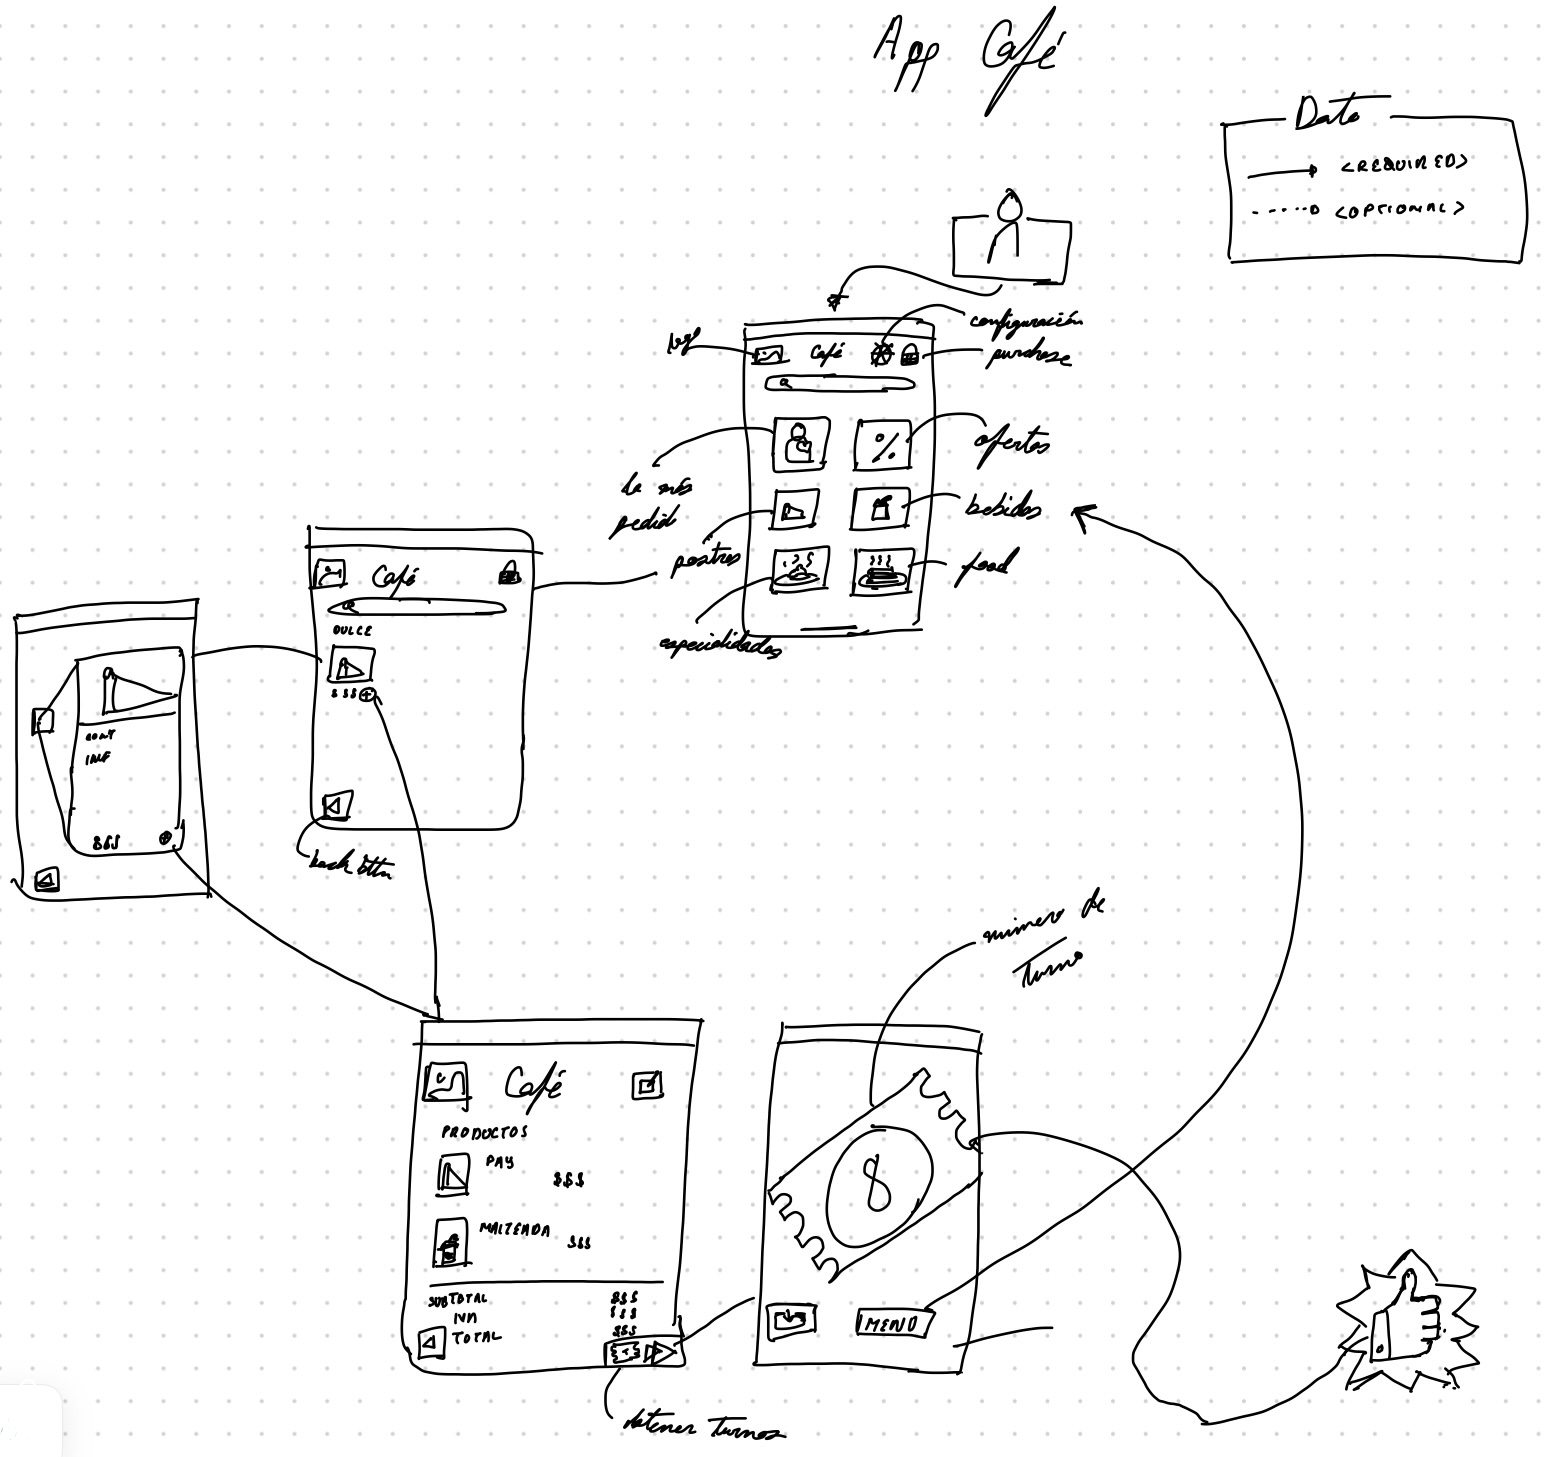
\includegraphics[width=0.035\textwidth]{./Assets/Img/Diagrama-cafe-app.jpg}
	\caption{Diagrama de flujo}
	\label{fig:Diagrama-cafe-app}
\end{figure}


\subsection {Flujo ideal}
\begin{itemize}
  \item Seleccionar una categor�a.
  \item Seleccionar un alimento.
  \item Agregar a la canasta.
	\item Revisar su pedido.
	\item Obtener tu turno.
\end{itemize}

\subsection {Flujo alterno}
\begin{itemize}
  \item Seleccionar una categor�a.
		\subitem Usar la barra de busqueda
		\subitem Revisar tu canasta.
  \item Seleccionar un alimento.
		\subitem Usar la barra de busqueda
		\subitem Revisar la informaci�n nutrimental del alimento.
		\subitem Ver resenas.
		\subitem Agregar el alimento a la canasta.
		\subitem Revisar la canasta.
		\subitem Regresar a la selecci�n de categor�as.
  \item Agregar a la canasta.
		\subitem Seguir comprando.
		\subitem Regresar a la selecci�n de categor�as.
		\subitem Revisar la canasta.
	\item Revisar su pedido.
		\subitem Regresar a la selecci�n de categor�as.
		\subitem Regresar a la selecci�n de alimentos.
	\item Obtener tu turno.
\end{itemize}

\end{document}